\chapter{系统设计}

\section{框架选型}

\subsection{LeapMotion 与 LeapJS}

\subsection{watchOS 与 WatchConnectivity}


\section{架构设计}
\label{sec:架构设计}

\subsection{通信架构}
\label{sub:通信架构}

watchOS 从 2.0 开始从 iOS App Extension 中剥离开来,将 Watch App 部分全部移至 watchOS 端,这时这部分代码在手表端具备了可执行的权限,因此将 watchOS 从 1.0 中的单向接收 iOS 端的系统级的通信,转变为第三方 App 执行管理\cite{WatchGuide:2016},如图 \ref{fig:watch-phone} 所示。这使其与外界的及时通信成为了可能。

\begin{figure}[H]
    \centering
    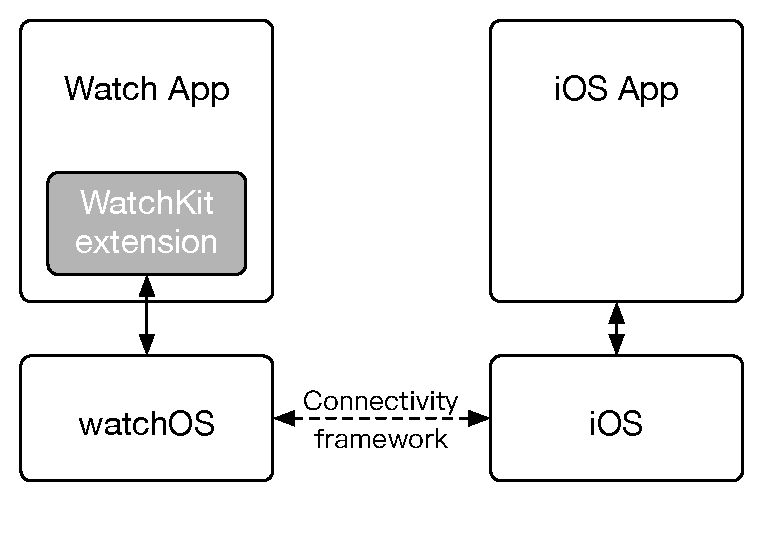
\includegraphics[width=0.4\textwidth]{figures/watch-phone}
    \caption{\kaishu Watch App、WatchKit 扩展和 iOS App 之间的联系}
    \label{fig:watch-phone}
\end{figure}

然而,即便如此在 watchOS 上的网络访问能力依然十分有限,在 watchOS 2 中\footnote{本文写成时的 watchOS 版本为 2.2。},Apple Watch 只能在和与其配对的 iPhone 失去连接,且同时处于已保存的 Wi-Fi 网络覆盖范围内时,才能独立使用 NSURLSession 访问网络,条件十分苛刻。

鉴于以上考虑,本文对从服务端到客户端的通信架构设计如图\ref{fig:im-arch}所示。

\begin{figure}[t]
    \centering
    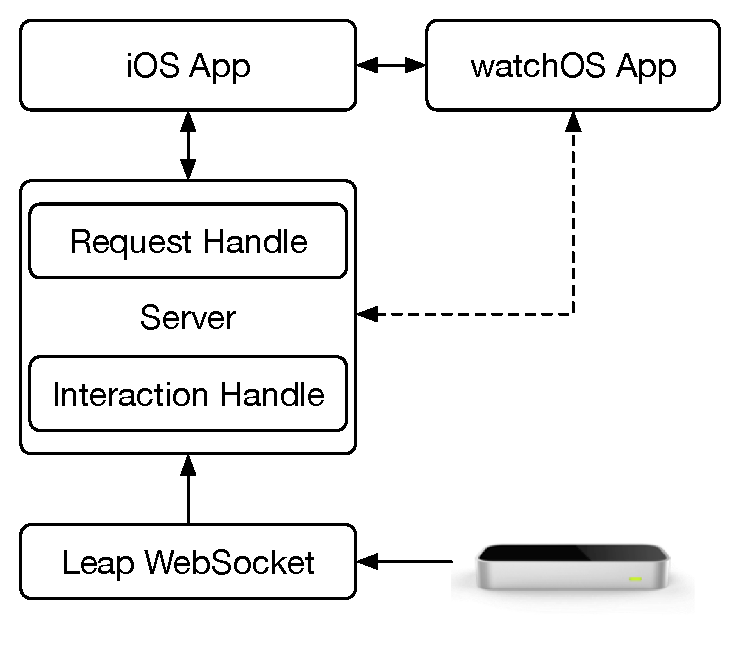
\includegraphics[width=0.4\textwidth]{figures/arch}
    \caption{\kaishu \textbf{通信架构}: watchOS 不直接与服务器进行通信,而是将 iOS 端作为与服务器通信的桥梁}
    \label{fig:im-arch}
\end{figure}

其中,watchOS 将 iOS 端作为与服务器通信的桥梁,处理性能及其有限的 watchOS 端仅负责对通信内容的呈献,性能稍强的 iOS 端对服务端消息进行筛选与加工,而服务端则对 LeapMotion 原始数据进行分析,并封装其分析结果后与 iOS 端进行通信。

\subsection{客户端架构}

\subsection{服务端架构}

\section{通信协议}

我们需要设计在 watchOS 和 iOS 之间、iOS 与 服务端之间设计相关的交互通信协议。

\section{演示程序}
